\documentclass{beamer}
\usepackage{times}
\usepackage{float}
\usepackage{graphicx}
\usepackage{color}
\usepackage{amssymb}  
\usepackage{soul}  
\usepackage{nameref} 
\usepackage{listings}
% wegen deutschen Umlauten
\usepackage[utf8]{inputenc}
% deutsche Silbentrennung
\usepackage[ngerman]{babel}
\usetheme{p2pframework}

\lstloadlanguages{Ruby}
\lstset{%
  basicstyle=\fontfamily{fi4}\selectfont\color{black},
  commentstyle = \fontfamily{fi4}\selectfont\color{red},
  keywordstyle=\fontfamily{fi4}\selectfont\color{blue},
  stringstyle=\color{green},
  language=Ruby,
  basicstyle=\footnotesize,      % font size
  numbers=left,                  % where to put line numbers
  numberstyle=\footnotesize,     % numbers size
  numbersep=5pt,                 % how far the line numbers are from the code
  backgroundcolor=\color{white}, % background color
  showspaces=false,                          % show spaces (with underscores)
  showstringspaces=false,            % underline spaces within strings
  showtabs=false,                            % show tabs using underscores
  frame=tb,                  % adds a frame around the code
  tabsize=2,                     % default tabsize
  breaklines=true,                  % automatic line breaking
  columns=fullflexible,
  breakautoindent=false,
  framerule=1pt,
  xleftmargin=10pt,
  xrightmargin=0pt,
  breakindent=0pt,
  resetmargins=true,
  stepnumber=1
}

\title{Systemanalyse und -design, Behaviour Driven Development}
\author[Steve Dierker]{dierker.steve@fu-berlin.de}
\date{\today}

\begin{document}

\frame{\titlepage}

\section{Gliederung}
  \begin{frame}{Gliederung}
    \begin{itemize}
      \item Was ist TDD?
      \begin{itemize}
        \item Begriffskl"arung
        \item Workflow
        \item Vorteile
        \item Probleme
      \end{itemize}
      \item Was ist BDD? 
      \begin{itemize}
        \item Workflow
        \item Demo
        \item Vergleich zu TDD
      \end{itemize}
      \item Andere Sprachen, andere Tools
    \end{itemize}
  \end{frame}

\section{Was ist TDD? - Begriffskl"arung}
  \begin{frame}{Was ist TDD? - Begriffskl"arung}
    \begin{itemize}
      \item TDD heisst Test Driven Development
      \item began 1998 mit Extreme Programming
      \item 'entdeckt' durch Kent Beck
      \item es ist ein Test-First Softwareprozess
      \item es gibt auch Test-Last Prozesse
    \end{itemize}
  \end{frame}

  \begin{frame}{Was ist TDD? - Workflow}
    \begin{center}
      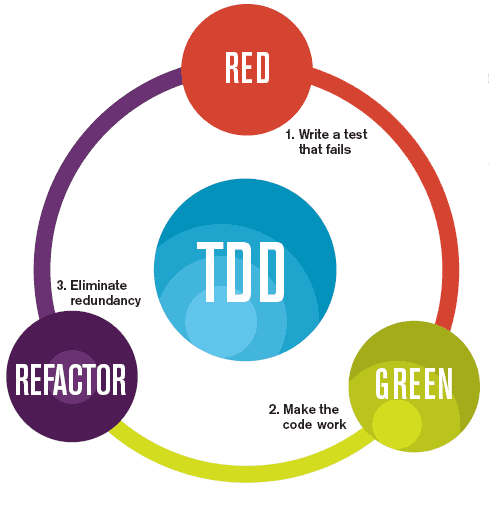
\includegraphics[scale=0.3]{../doc/assets/tdd_flow.png}
    \end{center}
  \end{frame}

  \begin{frame}{Was ist TDD? - Workflow}
    \begin{itemize}
      \item ein Zyklus sollte nicht l"anger als 15 Minuten dauern
      \item Debuggen schneller als neu implementieren?
      \item Features und Tests nicht zu gro"s w"ahlen
      \item nur ein Feature pro Test
      \item Refactor!
    \end{itemize}
  \end{frame}

  \begin{frame}{Was ist TDD? - Vorteile}
    \begin{itemize}
      \item es wird sich ein Emergentes Design bilden
      \item kompakt und minimalistisch
      \item kann sich dynamisch den Anforderungen anpassen
      \item erm"oglicht sofortiges Feedback
      \item immer begrenzt lauff"ahige Software
    \end{itemize}
  \end{frame}

  \begin{frame}{Was ist TDD? - Probleme}
    \begin{itemize}
      \item kein White-Box-Testing!
      \item keine Hinweise mit welchen Tests anzufangen ist
      \item was soll ueberhaupt getest werden?
      \item ersetz NICHT einen ausf"uhrlichen Testzyklus am Ende der Entwicklung
      \item Anforderungen m"ussen von Programmierer\_innen in Test "ubetragen werden
      \item kein Einheitliches Namensschema f"ur Tests
    \end{itemize}
  \end{frame}

  \begin{frame}{Was ist TDD? - Probleme}
    \lstinputlisting[caption=Ruby UnitTest,firstline=5,lastline=19]{../tests/calculator_test.rb}
  \end{frame}

  \begin{frame}{Was ist TDD? - Schlussfolgerung}
    \begin{itemize}
      \item Gute Idee, schwer zu vermitteln und zu meistern
    \end{itemize}
  \end{frame}


\section{Was ist BDD?}
  \begin{frame}{Was ist BDD? - Workflow}
    \begin{itemize}
      \item Erweiterung von TDD
      \item Stakeholder und Entwickler\_innen entwickeln Tests gemeinsam \( \rightarrow \) {\em Gherkin}
      \item Stakeholder und Enwickler\_innen benutzen die selben Tools
      \item ein weiterer Zyklus wird hinzugef"ugt
      \item But let's dive in!
    \end{itemize}
  \end{frame}

  \begin{frame}{Was ist BDD? - Workflow}
    \begin{center}
      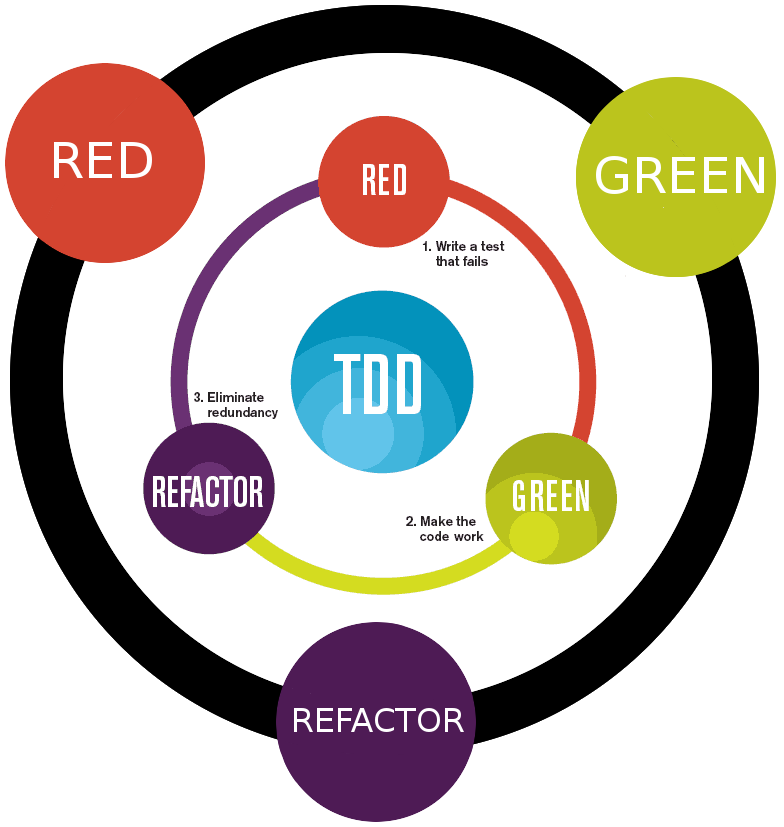
\includegraphics[scale=0.25]{../doc/assets/bdd_flow.png}
    \end{center}
  \end{frame}

  \begin{frame}{Was ist BDD? - Workflow}
    \lstinputlisting[caption=Cucumber Gherkin]{../features/addition.feature}
  \end{frame}

  \begin{frame}{Was ist BDD? - DEMO}
    \begin{itemize}
      \item Demo!
    \end{itemize}
  \end{frame}

  \begin{frame}{Was ist BDD? - Vergleich zu TDD}
    \begin{itemize}
      \item Stakeholder wird direkt an der Entwicklung beteiligt
      \item Fokus auf Verhalten der Software, allein durch Wortwahl
      \item Namenskonventionen
      \item automatisierte Dokumentation
    \end{itemize}
  \end{frame}

  \begin{frame}{Was ist BDD? - Vergleich zu TDD}
    \begin{itemize}
      \item bis jetzt keine Studien zu BDD
      \item Studien zu TDD:
      \begin{itemize}
        \item erh"oht Produktivit"at der Enwickler\_innen
        \item erh"oht Qualit"at der Software
        \item verbessert Design
        \item erh"oht Erweiterbarkeit der Software
        \item Schwierigkeiten in der Umsetzung
      \end{itemize}
    \end{itemize}
  \end{frame}

\section{Andere Sprachen, andere Tools}
  
  \begin{frame}{Andere Sprachen, andere Tools}
    \begin{itemize}
      \item Java \( \rightarrow \) \href{http://jbehave.org/}{JBehave}
      \item C \( \rightarrow \) \href{http://code.google.com/p/cbehave/}{CBehave}
      \item Ruby \( \rightarrow \) \href{http://cukes.info}{Cucumber}, \href{http://rspec.info}{RSpec}
      \item PHP \( \rightarrow \) \href{http://behat.org}{behat}
      \item Python \( \rightarrow \) \href{http://lettuce.it}{Lettuce}
    \end{itemize}
  \end{frame}

  \begin{frame}{Quellen}
    \begin{itemize}
      \item Dan North, Introducing BDD
      \item Scott Bellware, Behaviour-Driven Development
      \item Chelimsky, David and Dennis, Zach and Astels, Dave and Hellesoy, Aslak and Helmpamk, Bryan and North, Dan, The Rspec Book
      \item Diogo Osorio, Test Driven Development using PHPUnit
      \item Gherkin, https://github.com/cucumber/cucumber/wiki/Gherkin
      \item Cucumber, http://cukes.info/
    \end{itemize}
  \end{frame}

  \begin{frame}{Quellen}
    \begin{itemize}
      \item RSpec, http://rspec.info/
      \item Dan North, Introducing RBehave
      \item Kaufmann, Reid and Janzen, David, Implications of Test-Driven-Development
      \item Nagappan, Nachiappan and Maximilien, E. Michael and Bhat, Thirumalesh and Williams, Laurie, Realizing quality improvement through test driven development: results and experiences of four industrial teams
      \item David Janzen, Software Architecture Improvement
    \end{itemize}
  \end{frame}

\end{document}
